\chapter{Introducción}
\label{introduccion}

En la actualidad se disponen de dos líneas de extrusión encargadas de la producción del filamento de PLA (Poliácido láctico) que vende y distribuye la empresa bq. Este filamento, es usado en la actualidad como consumible para las impresoras 3D.\\

Cada línea de extrusión, está formada por los siguientes elementos:

\begin{itemize}
    \item \textbf{Extrusora:} Es la encargada de convertir la matería prima, que es introducida en forma de granza, a un hilo continuo denominado filamento. La granza son pequeños cilindros de PLA que son convertidos en filamento al salir de la extrusora.\\
    \begin{figure}[H]
    	\centering
    	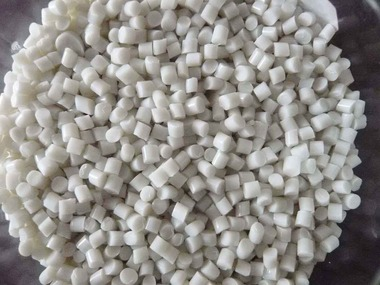
\includegraphics[width=0.3\textwidth]{images/PLA-Pellets.jpg}
    	\caption{PLA en forma de granza.}
    	\label{fig:intro_pellets}
	\end{figure}
    Explicado de una forma sencilla una extrusora es un tornillo sin fin dentro de un cañón calefactado que va fundiendo, mezclando y haciendo avanzar la granza, y posteriormente la masa a su través. En nuestro caso disponemos de cinco zonas de calentamiento para poder fabricar el filamento.\\
    \begin{figure}[H]
    	\centering
    	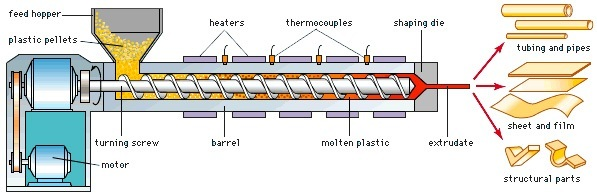
\includegraphics[width=0.9\textwidth]{images/Extruder.jpg}
    	\caption{Esquema de funionamiento de una extrusora.}
    	\label{fig:intro_extrusora}
	\end{figure}
    En la instalación sobre la que vamos a implementar el desarrollo contenido en este proyecto, la forma final es cilíndrica. Aunque existen multitud de modelos de boquilla para extruir el material con disintas formas. (Ver figura \ref{fig:intro_extrusora})
    \item \textbf{Enfriaminento por inmersión:} 
    A la salida de la extrusora se coloca una bañera de enfriamiento que, como su propio nombre indica, se encarga de enfriar el material de forma gradual
    Se usa una 'bañera' llena de agua con una temperatura controlada para lograr el enfriamiento del filamento según salga de la extrusora.
    Es un método habitual en este tipo de tecnología de fabricación debido a las altas velocidades de producción que podemos llegar a adquirir.
    \begin{figure}[H]
    	\centering
    	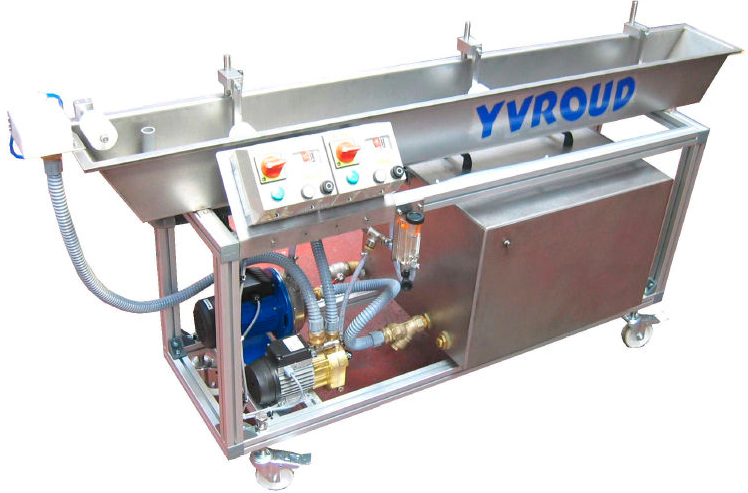
\includegraphics[width=0.6\textwidth]{images/enfriamiento.png}
    	\caption{Ejemplo de bañera usada en enfriamiento por inmersion}
    	\label{fig:intro_bañera}
	\end{figure}
    \item \textbf{Unidad tractora:} mediante la que se hace avanzar el filamento desde la salida de la extrusora hasta la entrada de la bobinadora. Siendo responsable del adelgazamiento del filamento, que aún se encuentra templado en la bañera de refrigeración.
    \item \textbf{Unidad de almacenamiento:} al tratarse de un proceso continuo es necesario un sistema que actue como buffer de filamento mientras se realiza el cambio de carrete en la bobinadora.
    \item \textbf{Bobinadora:} Es la encargada de enrollar el filamento en bobinas para su posterior distribución. Estás bobinas también son las usadas normalmente en la impresión 3D, aunque existe algún intento de estandarización al respecto, cada fabricante tiene su carrete. Y no todos son compatibles entre si. En esta parte de la instalación, es donde se tiene un control del diámetro final que adquiere el filamento, ya que es la última parte antes de su almacenaje.
    \begin{figure}[H]
    	\centering
    	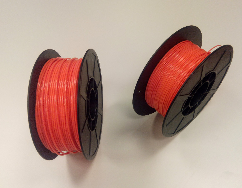
\includegraphics[width=0.4\textwidth]{images/carretes.png}
    	\caption{Carrete con filamento bobinado}
    	\label{fig:intro_carrete}
	\end{figure}
\end{itemize}

En la línea de fabricación existente la unidad tractora, la de almacenamiento y la bobinadora están integradas en una única máquina. En la actualidad el sistema es completamente funcional. Aunque los parámentros de entrada de cada uno de sus componentes (extrusora, bañera y bobinadora) se operan en lazo abierto y de forma manual. No es un producto adquirido de una vez. Por ello, no se dispone de comunicación directa, por ejemplo, entre la bobinadora y la velocidad de extrusión, en consecuencia, si hay algún tipo de error debe ser el operario encargado de la supervisión en parar todo el proceso y volver a arrancar.\\

La extrusión del filamento, es un proceso en el que influyen muchas variables como pueden ser la temperatura de la granza en el interior de la extrusora y la velocidad de extrusión. Estos problemas derivan en el producto final en que no se consigue un diámetro omogeno, en nuestro caso 1.75mm, como se puede comprobar en la imagen \ref{fig:muestra_filamento}.

   \begin{figure}[H]
        \centering
        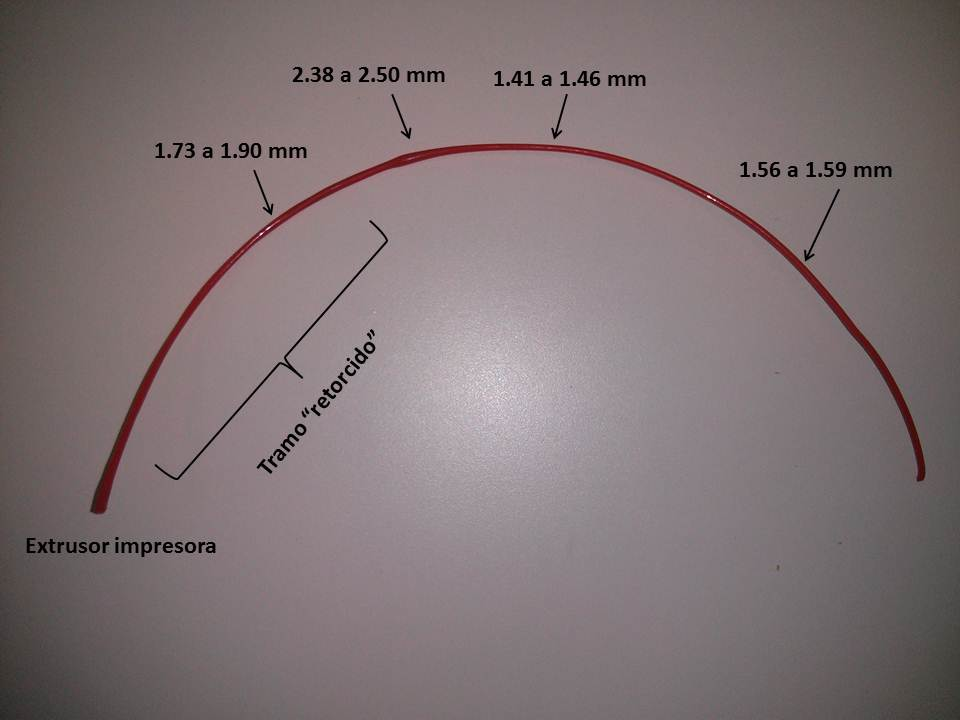
\includegraphics[width=0.45\textwidth]{images/atasco_rojo.jpg}
        \caption{Muestra de filamento con problemas en el diámetro}
        \label{fig:muestra_filamento}
    \end{figure}

